\documentclass[12pt,a4paper,table]{report}

\usepackage[utf8]{inputenc}
\usepackage{amsfonts}
\usepackage{amssymb}
\usepackage{setspace} 
\usepackage{graphicx}
\usepackage{array}
\usepackage{pdfpages}
\usepackage{mathtools}
\usepackage{hyperref}
\usepackage{nameref}
\usepackage{tabularx}
\usepackage[]{subcaption}
\usepackage[stable]{footmisc}
\usepackage{float}
%\usepackage[table]{xcolor}

%this is to make the \ref and \label command work at any text
\makeatletter
\let\orgdescriptionlabel\descriptionlabel
\renewcommand*{\descriptionlabel}[1]{%
  \let\orglabel\label
 \let\label\@gobble
 \phantomsection
  \edef\@currentlabel{#1}%
 \edef\@currentlabelname{#1}%
 \let\label\orglabel
  \orgdescriptionlabel{#1}%
}
\makeatother


\title{Valens - An Android application system to detect fall risk among the elderly}
\author{
  Vassdal, Johannes Willumsen\\
  \texttt{johannes.vassdal@gmail.com}
  \and
  Aamot, Elias\\
  \texttt{eliasaa@stud.ntnu.no}
  \and
  Larsen Tomren,Filip Andre\\
  \texttt{filip@tomren.it}
    \and
  Pham,Dat-Danny\\
  \texttt{datdanny@hotmail.com}
    \and
  K\"{u}c\"{u}kyareli,Tayfun\\
  \texttt{tayfun.kucukyareli@live.de}
}

\begin{document}
\onehalfspacing
\maketitle
\tableofcontents

\chapter{Introduction}

Damage from falling is the main cause for hospitalization among the elderly. In addition to the enormous costs incurred to society, falling is also the cause of great personal tragedy. As the use of computational devices becomes more common, it seems natural to examine how such devices can contribute to preventing such accidents.

This project is a cooperation between SINTEF and a group of students at NTNU for the course IT2901. Its goal is to develop a model for risk level of movement based on common sensors found in Android smart phones, and build an API to make the model accessible for third-party developers.

\section{Group introduction}
The group consists of 5 members, four of which were from Norwegian University of Science and Technology, and the remaining student was an exchange student from Germany, Technical University of Dortmund. The members had experience with programming and project development with the programming languages Java and C$  $, but little experience with Android applications. 

\section{Customer introduction}
The customer was "Selskapet for INdustriell og TEknisk Forskning ved norges tekniske hoegskole", or SINTEF for short. The person representing SINTEF was Babak A. Farshchian, Adjunct Associate Professor at NTNU. 
\chapter{Requirements}
\section{Understanding of requirements}

After first meeting with the customer we were told that we should not create a requirement specification right away because of the
way that the customer would like to work. The customer favours agile methods where the specification changes as we go along, and 
hence makes it difficult to write that much about.

But, from the project description we have that the students (we) will develop:
- A model of physical movements based on common movement sensors found in Android smart phones.
- An Android content provider that stores and makes available the data in this model through an API (content provider API).
- An example application that can visualize this data.

Our first requirements is to create scenarios for the overall product and paper mockups of the example application.
%\chapter{Alternative solutions}
This is where we mention where some alternative solutions to the problems we are tasked to solve. In particular describing the programs mentioned in the report written by Filip that is placed on Google drive and called "Alternative Solutions Report" or something similar.
%When that is done the above text needs to be commented or deleted

\section{Edmondo}

\section{Pedometer}
This is an app which focuses on giving the phone a pedometer function. This means to measure the number of steps taken while wearing the phone.
An open source app with a GPLv3 license that was compatible with the Apache 2.0 license used by the group. The app uses the same sensors that was needed to make the Fall-Prevention app work, and was therefore a good tool to learn and understand how such a thing could be done on Android. The licence compatability also means that anything of interest can be copied or studied as needed.


\section{GPS Status}
\chapter{Testing}
This chapter only touches the surface of general software testing, while focusing on methods, types and levels used in this project.
\section{Levels, methods and types}
Software testing is broken down into several levels, methods and types.
\subsection{Levels}
Software testing has four levels that correspond to how far into the software development process the team has come. The first three test levels refer to the development process and the last level refers to completion, or after development.
\begin{enumerate}
\item Unit testing is the first level where all individual components, such as functions, are tested. Often these tests are done by inputting sample data and validating output.
\item Inspections refers to a peer review or code review process where a team of individuals read through the source code to reveal early and obvious bugs. An error or bug that is not very visible for the developer may be very visible to an inspector.
\item Integration testing is the next step which takes groups of individual components to verify that they work together or to reveal faults in the integration.
\item System testing is the last step of test in the development process where the complete system or software is tested to evaluate it's match to it's requirements.
\item Acceptance testing is the last and highest level of testing where the system or software is tested to verify that it is acceptable for delivery. The test itself is usually Black Box Tests (see page \pageref{def:blackboxtesting}) to see if the customer will receive the desired and expected results.
\end{enumerate}
\subsection{Methods}
The approach to software testing is called methods or techniques. Primarily there are two methods when testing software; black box testing, and white box testing.
\begin{itemize}
\item \label{def:blackboxtesting} Black Box Testing is named so because the internals of the software or system is not visible to the tester, like inside a dark black box. The tests are usually functional tests to reveal interface problems, functionality flaws, performance troubles, behaviour errors and incorrect or missing functions. This test method is usually done by independent testers with no programming or implementation knowledge. Mainly these test method is applicable at a higher level of testing; System testing and Acceptance testing.
\item White Box Testing is a test method where the internals of a software or system is known to the tester, who usually is a programmer. Programming and implementation knowledge is required in this method since this method studies the code and goes way beyond the interface visible to the end user. The method is mainly applicable in lower levels of testing like Unit testing and Integration testing, but it is mostly used in Unit testing. The overall advantage of this test method is that testing can be started on in an earlier stage to make sure every bit of program produces correct output given an input and gives the opportunity to quickly correct problems.
\end{itemize}
\subsection{Types}
Only some of the test types are mentioned in this chapter, though there are many different testing types not used in this process and therefore not covered.
\begin{itemize}
\item Smoke Testing, only tests major functions of a software or system to decide if it further testing should proceed. If the Smoke Tests fail, no further testing is necessary due to deeper testing will fail. A kind of Smoke Test could be to check if the software compiles and starts up. Smoke Tests should under no circumstance replace Functional or Regression Testing.
\item Functional Testing, verifies if the software or system to have met its requirements or specifications. In functional testing, Black Box Testing is performed where the tester has no aspect of what is going on internally. See above explanation about Black Box Testing for more. When performing Functional Testing a set of inputs and expected outputs are matched up to one another, where they do not match the test fails. When performing this type of testing it is easy to miss logical errors due to the fact that the tester do not know what is going on underneath the code.
\item Regression Testing, essentially re-tests previously verified tests to ensure that bug fixes, enhancements or optimization has not affected the system or software after a given change in code. The test type can be performed on any level, but is mostly relevant on the System Testing level when the bug fixing, optimization and enhancements are done. Many companies choose to automate these tests to save time and money when software or systems has changed.
\end{itemize}
\section{Plans and process}
During the first period of development with the incremental process, test plans were not laid out due to the details of the process with no known end-results which would have added a lot of extra work redesigning testing plans after every customer meeting. After switching to agile development process testing got a lot more focus as described below.
\subsection{Unit testing}
Unit testing in the project was never done properly, nor properly documented. The method used was a form that adopted the essence of unit testing, and was done on-the-fly to verify that input correlated with output, and then removed. It was the most of the time done in-line and was not suited for reuse. Instead of heavy unit testing, it was partially replaced by Inspections.
\subsection{Inspections}
Inspections done in this project falls under the category "Code review" where part of the team or individuals read blocks of code to ensure its quality and to find bugs. A single developer working on a block of code can often get "blind", saying that they do not see obvious mistakes. Code review by a team member can speed up the process of identifying these bugs and defects for the developer to fix. This method became one of the most important types of testing to fry bugs in this project.
\subsection{Integration testing}
The integration of this project is divided into two levels; method- and system integration. Due to the fact that this project essentially consist of three standalone application every application was tested for themselves and then finally together.

The first integration testing was done for every application separately. This was done by just trying to run the application and checking the outcome after every run and was mostly done by the developer themselves. The reason to choose this kind of approach to this form of testing was the fact that an integration test plan takes time to write and every application was very compact with few functions. There are of course negative sides of this kind of approach that include lack of useful documentation, overlooking non-obvious failures and not knowing exactly how the final application should work. The alternative was to have a test plan worked out beforehand to follow and to explain all of this, but due to the lack of knowledge about testing and incremental processes this was neglected due to the reasons stated above.

The second part of integration testing was the system as a whole while developing. This was also done by just trying to run the applications and checking that the data flow between the applications worked. In this stage a form of smoke testing were used by checking if the data storage increased (data being saved to the phone) and by checking the output in the GUI app (statistics screen showing data).
\subsection{System testing}
System testing is the second to last level of testing, to verify that the system works together as a whole. In the project the system testing was done parallel to the last past of integration testing because of two reasons; time and complexity.\\

Since the app system consists of very few components the team decided to grasp the opportunity so save time and combining a few of the integration tests and system tests since they in essence overlapped each other.\\

The tests done in this stage is all done in the visible part of software, or also known as black box testing where you are blind to the code behind. Differing from previous methods, this part of testing had tests developed and laid out beforehand and all the faults, bugs and defects were noted according to these tests and afterwards fixed by a developer before commencing new tests. This because an error or bug may be connected and one bug can cause or solve another.
\subsection{Acceptance testing}
The last level before handing over the final application to the customer, but tested in a production environment. The same tests were performed as in the system testing level and bugs, faults and defects were again noted to be fixed before rolling out a new version for testing. After no tests failed the application were considered stable and delivered to the customer.

\subsection{Summary of interview with medical professionals}
This is a summary of the information gathered by a meeting with two medical professionals and the customer.
\textbf{Present:} All group members, Babak Farshchian, Jorunn L. Helbostad, Beatrice Vereijken \\
\textbf{Time:} 14.15-15.37\\
\textbf{Place:} St.Olavs Hospital\\
The plan was to have a short presentation, a short GUI demonstration, and then discuss and interview with the interviewees. \\
\subsubsection*{Feedback on Interface and Presentation of the program}
\begin{itemize}
\item Immediate and summarized feedback was desired, as it would be more helpful than feedback later.
\item A focus on falling is not a selling point, try health or lifestyle instead
\item Menu is not obvious to people without android experience
\item Interface seems too complex for target groups
\item Text might be too small
\item Graph needs more contrast 

\end{itemize}

\textbf{Feedback on program functionality}
\begin{itemize}
\item Feedback should be tailored to particular groups
\item Self-testing can be useful for reducing risk and keeping awareness,
\item Small tests to measure reaction time, for example reaction to light or sound
\item Researchers could also be interested in data gathering
\item Measuring transitions between sitting/lying and standing up
\item Compare behavior on a weekly basis will give an overview of whether things are good or not
\end{itemize}

\textbf{Feedback on medicinal stuff}
\begin{itemize}
\item Preventing inactivity over time is useful to reduce risk
\item People with stability problems increase risk when moving much
\item Variable gait pattern is useful for predicting risk
\item Step time is more robust (and hopefully easy to measure)
\item A common exercise is to take a step forwards, sideways, backwards, sideways (measuring a box)
\item People in risk group are those who cut out walking, taking the bus, want help from others around the house
\item Irregularity in speed and length is important to look for
\item Appropriate movement amount for gender and age group is usually known
\item Time needed to turn in place
\end{itemize}
\subsection{Informal usability test}
During the meeting with the medical experts, the group gave an small and informal usability test to the two experts. 

\textbf{Prototype test}\\
\textbf{Subjects: Beatrice \& Jorunn}
\\

\subsubsection{Procedure}
This test was mainly focused on how intuitive it was to navigate the application system and how easy it was to understand the data received by the system. The procedure for this was to give the test subject a phone with program installed. They would then be asked to accomplish a few short tasks, and the observers would rate how easy the subject accomplished the tasks. 

\subsubsection{Results}
The data received from the system was easy to spot and easy to understand. The subjects had some difficulty finding the menu button for the first time, but had no problems with using it later on. It was overall relatively easy to navigate the system. However, the complexity was likely to be a bit much for the target group.
\section{Tests used under development}
\label{tab:TestsStart}
Here goes the tests for the GUI and demo application:
\subsection{GUI Tests}
Here is the tests for the demo application and the GUI.
\begin{figure}
\small

\begin{tabularx}{\textwidth }{|l|X|}
\hline
\cellcolor{blue!25}\textbf{Info} & \cellcolor{blue!25}\\
\hline
\textbf{Title} &Activity start\\
\hline
\textbf{TestID} & 01\\
\hline
\textbf{Writer}& Johannes\\
\hline
\textbf{Developer}& Dunno\\
\hline
\textbf{Date created}& date test was planned\\
\hline
\textbf{Date tested}& date test was performed\\
\hline
\textbf{Tester}& Everyone\\
\hline
\textbf{Preceding test}& NA\\
\hline
\textbf{Test data} & Application and android phone or emulator \\
\hline
\end{tabularx}

\begin{tabularx}{\textwidth}{|X|X|X|X|X|X|}
\hline
\cellcolor{blue!25}&
\cellcolor{blue!25}Description&
\cellcolor{blue!25}Input data&
\cellcolor{blue!25}Expected result&
\cellcolor{blue!25}Real result&
\cellcolor{blue!25}Status\\
\hline
\textbf{Step 1} & Start up application in phone or emulator & Nothing, just program start & Write name screen & Write name screen shows up & Correct!\\
\hline
\textbf{Step 2} & Write name in name box and click OK & A valid name & Greeting with name & Greeting with name & Correct!\\
\hline
\end{tabularx}
\label{fig:test01}
\end{figure}

\begin{figure}
\small

\begin{tabularx}{\textwidth }{|l|X|}
\hline
\cellcolor{blue!25}\textbf{Info} & \cellcolor{blue!25}\\
\hline
\textbf{Title} & Event list and details\\
\hline
\textbf{TestID} & 02\\
\hline
\textbf{Writer}& Johannes\\
\hline
\textbf{Developer}& Dunno\\
\hline
\textbf{Date created}& dunno\\
\hline
\textbf{Date tested}& dunno\\
\hline
\textbf{Tester}& Everyone\\
\hline
\textbf{Preceding test}& Test 01\\
\hline
\textbf{Test data} & Notifications stored in database \\
\hline
\end{tabularx}

\begin{tabularx}{\textwidth}{|X|X|X|X|X|X|}
\hline
\cellcolor{blue!25}&
\cellcolor{blue!25}Description&
\cellcolor{blue!25}Input data&
\cellcolor{blue!25}Expected result&
\cellcolor{blue!25}Real result&
\cellcolor{blue!25}Status\\
\hline
\textbf{Step 1} & User tries to access notifications  & User clicks smiley face & List of notifications is displayed & List of notifications is displayed. & Correct!?\\
\hline
\textbf{Step 2} & User clicks on notification title & User click and database input & Detailed view of notification & Detailed view of notification&Correct!\\
\hline
\end{tabularx}
\label{fig:test02}
\end{figure}
% template 
%\begin{tabular}{|l|l|}
%\hline
%\cellcolor{blue!25}\textbf{Info} & \cellcolor{blue!25}\\
% \hline
%\textbf{Title} & Motta moteinnkalling\\
%\textbf{TestID} & 6\\
%\textbf{Writer}&\\
% 
%\textbf{Developer}&\\
% 
%\textbf{Date created}& 28.02.2013\\
%\textbf{Date tested}&\\
%\hline
%\end{tabular}
%\begin{tabular}{|l|p{5cm}|}
%\hline
%\cellcolor{blue!25}\textbf{Requirements}&\\
% \hline
%\textbf{Preceding test}& 5. Kalle inn til møte\\
%\textbf{Test data} &Bruker registrert i systemet, avtale registrert i system, møteinnkalling er laget.\\
%\hline
%\end{tabular}


\chapter{Project Management}
\section{Development process}
The Customer wanted to give the developers small tasks from week to week, which resembles a inkrementall system development method.
In the first week the developers were given the task to make a mock-up of the project. They were later on asked to develop a prototype og the mock-up.
It was decided by the developers that they would have online meetings twice a week and an offline meeting once a week. 
The working hours was set to not less than 20 hours a week, but the developers was free to choose when to work themselves.
\section{Team Roles and Organization}
A description of your team organization - Roles and responsibilities,
 

\chapter{Development Environment}

\section{Code-sharing}
It was requested that the group would use the tool Github to share code and perform version control. Github had browser-based interfaces and downloadable clients, meaning all the members of the group could make use of it. \\
The repository that was to be used for the project was called "Fall\_Prevention\_2013". The first content shared in the repository was this report, in form of .tex files and a .pdf. Later this repository would also be used to keep the code in order. 

\section{IDE}
The demands from the IDE was as following:
\begin{itemize}
\item Could be used with Android programming
\item Was sufficiently understood by the team members to be used
\end{itemize}
To fill these requirements, and because there was plenty of tutorials that could be found, the group decided to use the Eclipse IDE, with add-on's to more easily code and deploy towards Android. 

\section{Prototyping}
Graphical prototyping was done with a service called "proto.io" and with paper scetches. The scetches were subsequently shown to the group and the customer. 
\chapter{Implementation}
\section{Plans}


Nearing the end of every spring, the customer and group agreed upon the content of the following sprint. 

<<<<<<< HEAD

\begin{tabular}{|c|c|p{6cm}|}
\hline
Sprint nr. & Date & Summary\\
\hline
Sprint 1: & 03.02.13 - 08.02.13 & Developing user stories and paper prototypes of the GUI.\\ 
\hline
Sprint 2: & 08.02.13 - 15.02.13 & Developing a mock-up application demonstrating the GUI.\\
\hline
Sprint 3: & 15.02.13 - 22.02.13 & Improving UI and functionality for the prototype, researching medicinal factors. \\
\hline

\end{tabular} 

 






\section{Architecture}
The application is made in a way that is common for all android applications. This means that
\begin{description}
\item[User interface] is described in xml layout files that is called in java code. Strings and resources is placed in a separate folder and file, to be accessed by the code as needed. This is to separate content and layout in the UI.
\end{description}
\subsection{}
=======

\begin{tabular}{|c|c|p{6cm}|}
\hline
Sprint nr. & Date & Summary\\
\hline
Sprint 1: & 03.02.13 - 08.02.13 & Developing user stories and paper prototypes of the GUI.\\ 
\hline
Sprint 2: & 08.02.13 - 15.02.13 & Developing a mock-up application demonstrating the GUI.\\
\hline
Sprint 3: & 15.02.13 - 22.02.13 & Improving UI and functionality for the prototype, researching medicinal factors. \\
\hline

\end{tabular} 

 

\section{Results}
\subsection*{Second mockup}
After the second meeting with the customer, the group had a sketch that was to be used as a starting point for the mock-up application. \\
\setlength\fboxsep{0pt}
\setlength\fboxrule{1pt}
\fbox{\includegraphics[trim = 20mm 180mm 0mm 20mm, clip, width=\linewidth]{Res/mockupV2}}
>>>>>>> 3df7106e49e80e13184c59f32b7f4cf3dbce3e50



\chapter{Research and Alternate Solutions}
A significant part of the planning phase for the project consisted of research. Two areas which required research were identified:
\begin{description}
\item[Domain knowledge:] No member of the group had any familiarity with the application domain, neither with the specific domain (fall studies) nor any of the related domains (like healthcare, medicine or sport science). A basic understanding of the domain is critical for communication with the expert group, as well as for the ability to develop and assess solutions independently of the expert group.
\item[Related software:] Related applications function as sources of inspiration, proofs of what is feasible to implement or even as aids during programming. Open source software can be partially or entirely incorporated into the code. Knowledge of related software can thus increase development efficiency.  
\end{description}
For each of the two areas of research, one member of the group was assigned to research and compile a concise report, so that the rest of the group could efficiently attain the required knowledge.   

The two reports will be reproduced in the following sections.

\section{Falling: Causes, Consequences and how to avoid it}
This report collected information from several sources on the subject of falls among the elderly. Particular focus is given to risks and avoidance strategies.

\subsection{Risk factors}
There are several factors that predicate risk of falling. Typical risk factors are:
\begin{itemize}
\item 
\textbf{Biological risk factors (sorted by order of significance):  \cite{fallsRubenstein}}
\begin{itemize}
\item Muscle weakness
\item Balance deficit
\item Gait deficit
\item Visual deficit
\item Mobility limitation
\item Cognitive impairment
\item Impaired functional status
\item Postural hypertension
\end{itemize}
\item 
\textbf{Behavioral risk factors(Not in sorted order):}
\begin{itemize}
\item Inactivity \cite{cdcComProg}
\item Medications \cite{cdcComProg}
\item Alcohol use \cite{cdcComProg}
\item Living alone \cite{housing}
\end{itemize}
\item 
\textbf{Home/environmental risk factors(not in sorted order): \cite{WHO}}
\begin{itemize}
\item Bad footwear or clothing.
\item Dangers in the house or in public places.
\item Unfamiliarity with walking aids such as canes, crutches, walking chairs.
\end{itemize}
\end{itemize}

A fall is normally caused by the interaction of two or more of these risk factors, but home or environmental risk factors cause only 30-50\% of all falls\cite{fallsRubenstein, cdcComProg}. What this means is that more than half of all falls happen without any influence of environmental factors. Also, in most of these cases where external factors play a role, the fall is in reality caused by an interaction between these and physiological aspects. The second and third most common single causes of falling are gait/balance disorders and dizziness/vertigo, followed by \emph{drop attacks}, which are sudden falls without loss of consciousness or dizziness\cite{fallsRubenstein}. As the project task is to develop a model for physical movement, it might be necessary to down-prioritize identifying risk for dizziness/vertigo and drop attacks, as well as ignore external factors, in order to focus purely on physiological aspects, such as gait or balance.

Many older adults are unaware of their risk factors, and therefore unable to take preventive actions. Even older adults with a history of falling have normally been given little education about the potential risk factors. Any sort of risk assessment, is therefore be very beneficial, especially when the results are discussed with a healthcare provider\cite{cdcComProg}. This fact illustrates the usefulness of the planned application. 

It has been shown that many of the biological risk factors can be reduced effectively by preforming regular physical activities. Specifically strength, gait and balance has been shown to be improvable by simple exercise regimes - even for frail patients - in a number of studies\cite{LMTassessPrev, cdcComProg, WHO}. A potential focus area for the app can therefore be encouraging exercise and healthy lifestyles.

\subsection{Advice for prevention}
The individual can easily reduce the risk of falling greatly by taking certain measures. A list of measures normally, by the authorities, recommended for older people in the target group is given below\cite{cdcYouPrevent}:

\begin{itemize}
\item Begin a regular exercise program.
\begin{itemize}
\item Exercises that improve balance and coordination are the most helpful.
\item Is the only measure that by itself reduces the risk of falling independently of individual circumstances. 
\end{itemize}
\item Have your health care provider review your medicines, even over-the-counter ones.
\begin{itemize}
\item Avoid medicines that can make you dizzy or sleepy.
\end{itemize}
\item Have your vision checked.
\item Make your home safer.
\begin{itemize}
\item Remove or fasten small rugs and carpets.
\item Remove wires and cords away from commonly taken paths. Tape wires to the walls, and if necessary install an additional power outlet.
\item Keep items where you can reach them without having to climb. If you have to use a step stool, get a stable one with handrails.
\item Remove loose items that can make you trip (books, papers, clothes, etc.) from the floor and stairs.
\item Add grab bars and non-slip mats to the bathroom.
\item Make your home brighter.
\item Repair broken or uneven steps and handrails in the staircase.
\item Avoid using the staircase more than necessary, for instance by installing a light switch at the top as well as the bottom of the stairs. 
\item Wear shoes, even inside. Avoid walking barefoot or wearing slippers.
\end{itemize}
\end{itemize}

\subsection{Physiological aspects}

The list below explains the physiological factors that contribute to stability. “A marked deficit in any one of these factors may be sufficient to increase the risk of falling; however, a combination of mild or moderate impairments in multiple physiological domains also may increase the risk of falling. By directly assessing an individual's physiological abilities, intervention strategies can be implemented to target areas of deficit.” \cite{LMTassessPrev}

\begin{itemize}
\item Reaction time
\begin{itemize}
\item Hand
\item Foot
\end{itemize}
\item Vision
\begin{itemize}
\item Contrast sensitivity
\item Visual acuity
\end{itemize}
\item Vestibular function
\begin{itemize}
\item Visual field dependence
\end{itemize}
\item 
Peripheral sensation
\begin{itemize}
\item Tactile sensitivity
\item Vibration sense
\item Proprioception
\end{itemize}
\item Muscle force
\begin{itemize}
\item Knee flexion
\item Knee extension
\item Ankle dorsiflection
\end{itemize}
\end{itemize}


There exists an array of tests that can measure the performance on these aspects. Lord et al. \cite{LMTassessPrev} provides one possible set of tests. Some of these are possible to implement in an app, but none of them are based on hip movement.

The test developed by Lord et al. \cite{LMTassessPrev} was used to classify older adults into fallers or non-fallers, and has an accuracy of $75-80\%$ in different experiments. If a test which disregards hip movement patterns performs well, there may be reasons to believe that hip movement is only a minor factor in detecting fall risk. However, 

Walking behaviour seems to be generally associated with falling. Lord et al. \cite{LLKgaitPatterns} shows that there is a negative correlation between falling and steps per minute, stride length and stride velocity. A positive correlation was shown between falling and stance duration and stance percentage. However, these physiological traits are all associated with old age, and old age is associated with falling, so the relation might be quite indirect. On the other hand, stride and stance as physiological aspects that can be measured with relative ease using a mobile phone.

\section{Related Applications}
There exist several other open source programs and commercial programs that solve related problems. These could function as inspiration for design, interfaces and functions, and open source programs can be imported and incorporated into the project. The most relevant related applications are presented below.

\subsection{Endomondo Sports Tracker}
This is a popular app for exercising. It can be used to track routes, times and progress in training and activities. It uses GPS (and accelerometer) to find position on maps and track the location. Very easy to use, and automatically syncs up to endomondo.com. Has an inspiring design and sync-functionality.

The main part of Endomondo is the inspirational part to get people to move; you can compare yourself to others, e.g. friends, and you have a really easy way to see what an exercise is worth in amount of calories and amount of burgers burned by an exercise.

A lot of aspects from this app can be used during design, especially labelling and representation of data.

\subsection{GPS Status}
This application is used to view detailed status about the GPS system on the phone. It has a very advanced interface with lots of numbers to show information, but for a rookie user the data rarely translates into information.

The app succeeds to use the sensors very heavily.

\subsection{Pedometer\footnote{Application can be found at \url{https://code.google.com/p/pedometer/}}}
An open source app that has a GPLv3 license that is compatible with our Apache 2.0 license. The app uses the same sensors that may be useful for the current project. Taking advantage of this could reduce development cost drastically.

The creator's description of how the step detection algorithm works\footnote{Taken from the FAQ at \url{https://github.com/bagilevi/android-pedometer}}: \textit{``Basically, it aggregates the sensor values, finds the maximum and minimum, and if the difference is bigger than a value (which depends on the sensitivity setting) then it counts it as a step. There's is some additional optimization, which I arrived to through experimentation."}\footnote{Taken from the FAQ at \url{https://github.com/bagilevi/android-pedometer}}

\subsection{GPS Tracker\footnote{Application can be found at: \url{https://code.google.com/p/open-gpstracker}}}
This program adds the capability to store and review where you and your Android device have been. Basically you press record at the start of your trip and your phone stores the route you take. This route is drawn real-time on the Maps functionality of Android or in the background with an idle device. The route is stored on your phone for review and further use. The applications tracks location by GPS, hence the name. An accurate description of the program type would be a GPS logger.

It contains the ability to log location, something that might prove useful for current project. Since it is open source and has a compatible license (GNU v3), it can be incorporated easily.

\subsection{Summary of interview with medical professionals}
This is a summary of the information gathered by a meeting with two medical professionals and the customer.
\textbf{Present:} All group members, Babak Farshchian, Jorunn L. Helbostad, Beatrice Vereijken \\
\textbf{Time:} 14.15-15.37\\
\textbf{Place:} St.Olavs Hospital\\
The plan was to have a short presentation, a short GUI demonstration, and then discuss and interview with the interviewees. \\
\subsubsection*{Feedback on Interface and Presentation of the program}
\begin{itemize}
\item Immediate and summarized feedback was desired, as it would be more helpful than feedback later.
\item A focus on falling is not a selling point, try health or lifestyle instead
\item Menu is not obvious to people without android experience
\item Interface seems too complex for target groups
\item Text might be too small
\item Graph needs more contrast 

\end{itemize}

\textbf{Feedback on program functionality}
\begin{itemize}
\item Feedback should be tailored to particular groups
\item Self-testing can be useful for reducing risk and keeping awareness,
\item Small tests to measure reaction time, for example reaction to light or sound
\item Researchers could also be interested in data gathering
\item Measuring transitions between sitting/lying and standing up
\item Compare behavior on a weekly basis will give an overview of whether things are good or not
\end{itemize}

\textbf{Feedback on medicinal stuff}
\begin{itemize}
\item Preventing inactivity over time is useful to reduce risk
\item People with stability problems increase risk when moving much
\item Variable gait pattern is useful for predicting risk
\item Step time is more robust (and hopefully easy to measure)
\item A common exercise is to take a step forwards, sideways, backwards, sideways (measuring a box)
\item People in risk group are those who cut out walking, taking the bus, want help from others around the house
\item Irregularity in speed and length is important to look for
\item Appropriate movement amount for gender and age group is usually known
\item Time needed to turn in place
\end{itemize}


\chapter{Conclusion}
In this chapter will have information concluding the project, such as what the group learned and experienced.
\section{New Experiences}
All members of the group has learned much about teamwork, project management, planning, programming in a group, programming towards the Android platform, programming documents in LaTeX, and writing documentation for project activities. 
\section{Learning experiences from development and tool use}
Following are things that relate to project management and software development that the group learned during the project:
\begin{itemize}
 \item  It is important to ensure that documentation is done in a systematic fashion. In the beginning, a large amount of the reports and documentation that the group made for internal use, turned out to create more work and confusion later on. This was in part because it was not thought to be necessary at the time. Looking back, it seems like it would have been much more efficient to write reports well, and write them in LaTeX  while they were still new.
 \item Communication and what tools to use, was in flux for some time. Even when a few tools were settled on, the group still had problems with making sure all the members were on the same page regarding what needed to be done. 
 \item  Usage of tools which not all members were equally experienced with turned out to be problematic. This was because of misunderstanding and difficulties which could often be resolved by only one or two members, and slowed down the entire group. This might have been mitigated if all the members had a better understanding of the tools that were used. This could be accomplished by teaching sessions and group members being encouraged to seek a better understanding on their own.
 \end{itemize} 
 

\section{Lessons learned about Research and Prestudies}
The research provided significant benefits for the group by providing a solid knowledge base for the application domain, so time spent on research was well spent. However, in retrospect the group was able to identify some faults in their research planning, and learned some lessons about how to avoid the same mistakes in the future:

\begin{itemize}
\item
Even though the research were accurate, the group was reluctant to employ the research results in the application before they were confirmed by the health experts. As the meeting with the health experts did not take place before 22.03, the group lost valuable time waiting, time that could have been spent for implementation. The lesson learned is to rely on research results, at least until a more reliable source of information is available (in this project, the expert group).
\item
Even though research was useful in the domains that were covered, some areas that could have benefited from research were not identified during planning, and were therefore not given thorough research. Because of this, some of the customer's demands were misinterpreted at first, forcing the group to change the application architecture at a later stage. In particular, the group was unfamiliar with the standards of Android development, especially the general architecture of Content Provider. A solid foundation in this area could have aided understanding. The lesson learned is to spend more time trying to identify potential research areas. 
\end{itemize}
\begin{thebibliography}{99}
%in case of citations, write \cite{title}in the relevant place
%and \bibitem{title}description 
%here
\bibitem{fallsRubenstein}
"Falls in older people: epidemiology, risk factors and strategies for prevention". Laurence Z. Rubenstein. Age and Ageing 2006; 35-S2:ii37-ii41.
\bibitem{LMTassessPrev}
"A physiological Profile Approach to Falls Risk Assessment and Prevention", Stephen R. Lord,Hylton B. Menz and Anne Tiedemann, Journal of the American Physical Therapy Association. 
\bibitem{LLKgaitPatterns}
"Sensori-motor Function, Gait Patterns and Falls in Community-dwelling Women". Stephen R. Lord, David G. Lloyd, Sek Keung Li. Age and Ageing 1996:25:292-299.
\bibitem{cdcYouPrevent}
	"What you can do to prevent falls", Centers for Disease Control and Prevention.
\bibitem{cdcComProg}
	"Preventing Falls: How to Develop Community­based Fall Prevention Programs for Older Adults", Centers for Disease Control and Prevention.
\bibitem{housing}
"Muscle strength, activity, housing and the risk of falls in elderly people." Wickham C et al., Age and ageing, 1989, 18:47-51 
\bibitem{WHO}
What are the main risk factors for falls among older people and what are the most effective interventions to prevent these falls? Todd C, Skelton D. (2004) Copenhagen, WHO Regional Office for Europe 
 
\end{thebibliography}

\appendix

\chapter{WBS}

\section{Previous WBS}
This is where the Work Breakdown Structures from early development is placed here with the most recent placed earliest, as can be seen in Figures \ref{fig:WBS222}, \ref{fig:WBS13}, \ref{fig:WBS83}, \ref{fig:WBS153}, \ref{fig:WBS223}, \ref{fig:WBS54}, and \ref{fig:WBSfin}.

\begin{figure}[p]
\setlength\fboxsep{0pt}
\setlength\fboxrule{1pt}\noindent\makebox[\textwidth]{%
 \fbox{
\includegraphics[width=1.45\textwidth , angle=270]{Res/WBSfirst.png}}}
\caption{The WBS as per 22.2.13 }
\label{fig:WBS222}
\end{figure}

\begin{figure}[p]
\setlength\fboxsep{0pt}
\setlength\fboxrule{1pt}\noindent\makebox[\textwidth]{%
 \fbox{
\includegraphics[width=1.45\textwidth , angle=270]{Res/WBS01313.png}}}
\caption{The WBS as per 1.3.13}
\label{fig:WBS13}
\end{figure}


\begin{figure}[p]
\setlength\fboxsep{0pt}
\setlength\fboxrule{1pt}\noindent\makebox[\textwidth]{%
 \fbox{
\includegraphics[width=1.45\textwidth , angle=270]{Res/WBS08313.png}}}
\caption{The WBS as per 8.3.13}
\label{fig:WBS83}
\end{figure}

\begin{figure}[p]
\setlength\fboxsep{0pt}
\setlength\fboxrule{1pt}\noindent\makebox[\textwidth]{%
 \fbox{
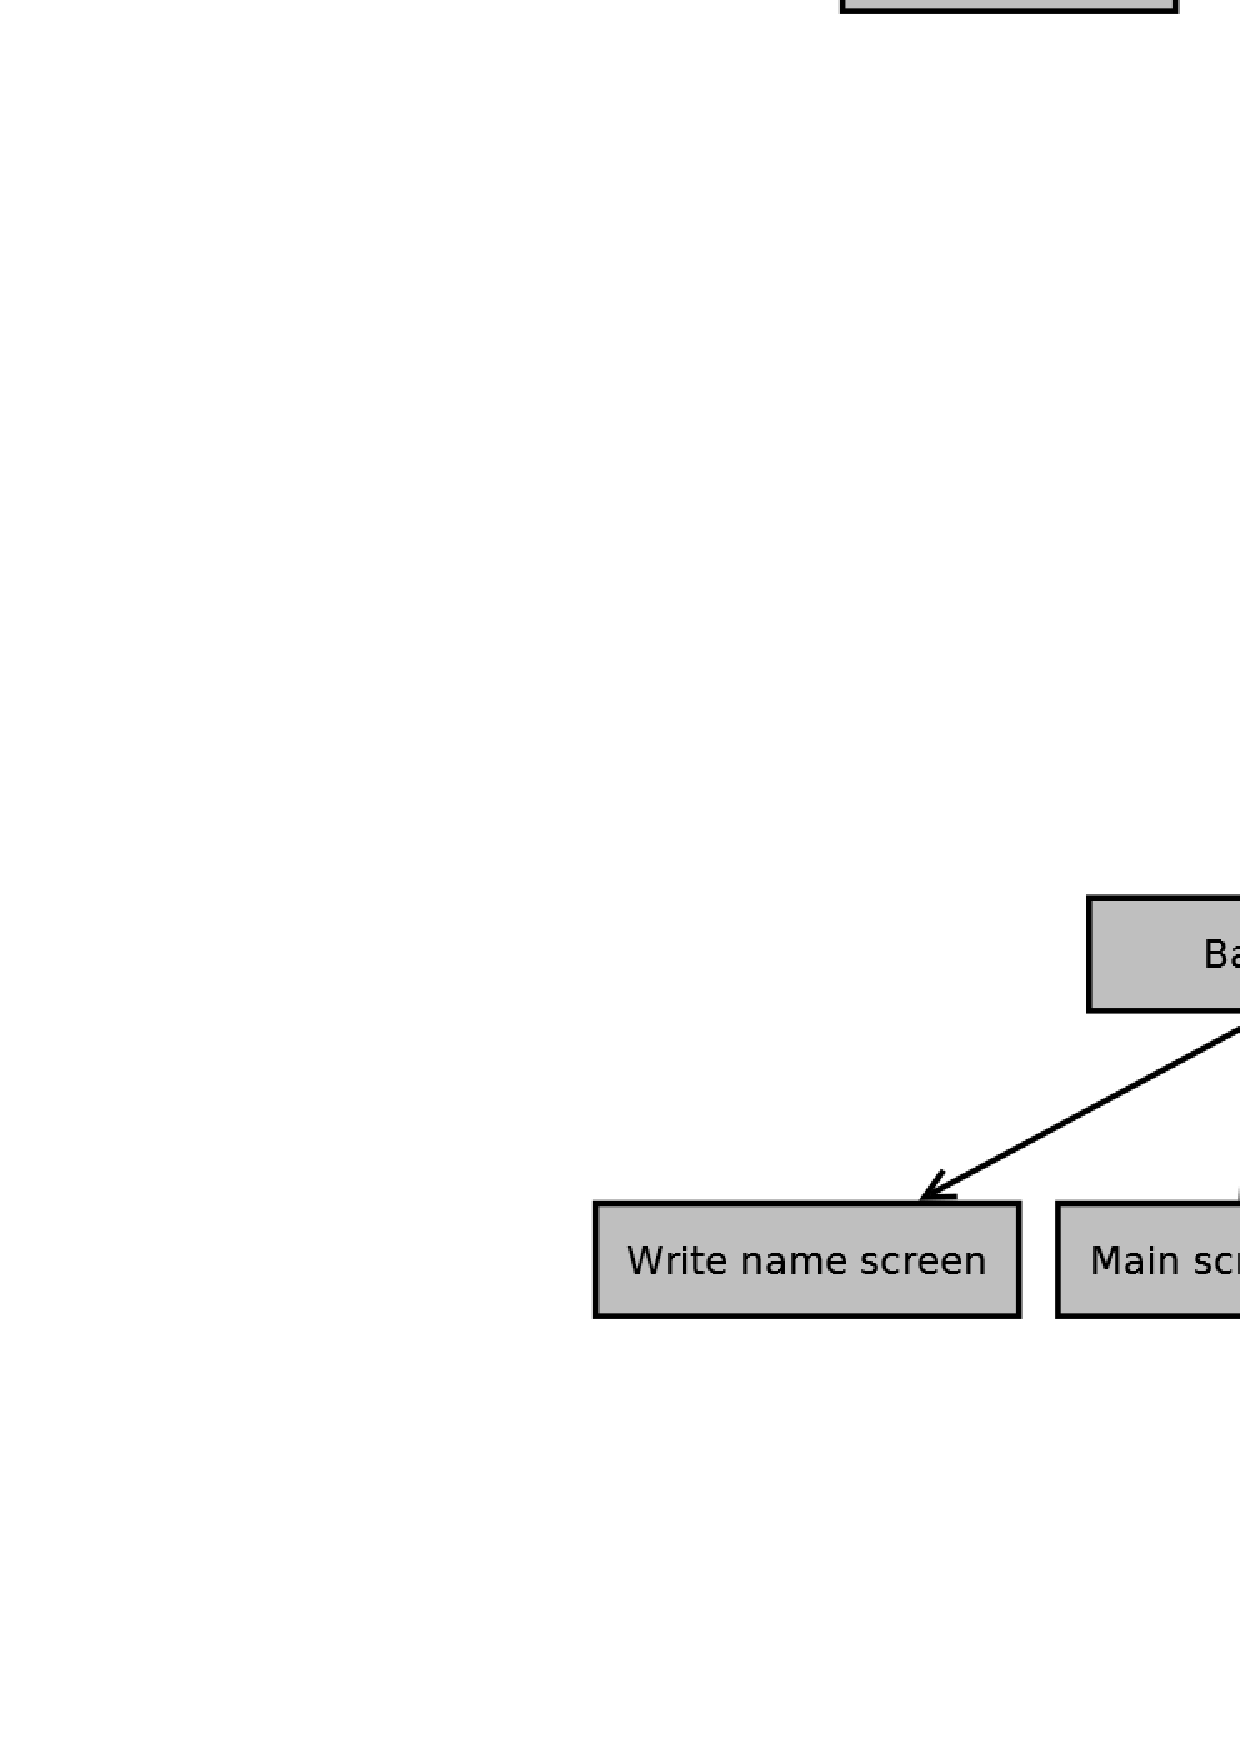
\includegraphics[width=1.45\textwidth , angle=270]{Res/WBS15313.png}}}
\caption{The WBS as per 15.3.13}
\label{fig:WBS153}
\end{figure}

\begin{figure}[p]
\setlength\fboxsep{0pt}
\setlength\fboxrule{1pt}\noindent\makebox[\textwidth]{%
 \fbox{
\includegraphics[width=1.45\textwidth , angle=270]{Res/WBS22313.png}}}
\caption{The WBS as per 22.3.13}
\label{fig:WBS223}
\end{figure}

\begin{figure}[p]
\setlength\fboxsep{0pt}
\setlength\fboxrule{1pt}\noindent\makebox[\textwidth]{%
 \fbox{
\includegraphics[width=1.45\textwidth , angle=270]{Res/WBS05413.png}}}
\caption{The WBS as per 5.4.13}
\label{fig:WBS54}
\end{figure}

\begin{figure}[p]
\setlength\fboxsep{0pt}
\setlength\fboxrule{1pt}\noindent\makebox[\textwidth]{%
 \fbox{
\includegraphics[width=1.45\textwidth , angle=270]{Res/WBSlast.png}}}
\caption{The final WBS}
\label{fig:WBSfin}
\end{figure}

%\section{Reports}

\chapter{Work summary}
\section{Sprint summaries}
\label{tab:sprintList}
The following is a list of the sprints:

\begin{description}
\item[Sprint 1: 01.02.13 - 08.02.13] \hline \hfill \\
User stories and paper prototypes of the GUI were developed.
\item[Sprint 2: 08.02.13 - 15.02.13] \hline \hfill \\
The group focused on learning Android development. New GUI paper prototypes were developed based on customer feedback. A mock-up application demonstrating core parts of the GUI was developed.
\item[Sprint 3: 15.02.13 - 22.02.13] \hline \hfill \\
Continued efforts on learning Android development. The mock-up was developed further. Research was conducted on the application domain, and on related applications. 
\item[Sprint 4: 22.02.13 - 01.03.13] \hline \hfill \\
The prototype application was expanded with a database, GUI visuals were improved, menu usage was made consistent throughout the prototype. The group tried to familiarize themselves with Content Providers in Android.
\item[Sprint 5: 01.03.13 - 08.03.13] \hline \hfill \\
A Content Provider was developed, incorporated the step detection from the Pedometer open-source application. Some secondary screens (settings and statistics) were implemented. Basic widget created.
\item[Sprint 6: 08.03.13 - 15.03.13] \hline \hfill \\
Widget was connected successfully to the main application. Application connected to the Content Provider. Work on report for the mid-term hand-in. Presentation for the focus group prepared. Unsuccessful attempts at making the Pedometer/Content Provider location aware. Implementation of contact management. 
\item[Sprint 7: 15.03.13 - 22.03.13] \hline \hfill \\
Research and development of step detection algorithm: Sensor data collection application developed, python scripts for displaying data and prototyping of algorithm. Work on Javadoc and code re-factoring. Correction of report based on mid-term feedback.
\item[Ester holidays: 23.03.13 - 02.04.13] \hline \hfill \\
Little work was done due to the holidays.
\item[Sprint 9: 03.04.13 - 05.04.13] \hline \hfill \\
New system architecture was designed. Step detection algorithm implemented as Android application. The old Content Provider/Pedometer discarded, and new Content Provider implemented. 
\item[Sprint 10: 05.04.13 - 12.04.13] \hline \hfill \\
Efforts were focused on bug-fixing and integration of the three components. 
\item[Sprint 11: 13.04.13 - 19.04.13] \hline \hfill \\
Work on final report and small adjustments the integration of the components. The code underwent re-factoring and commenting. 
\end{description}
\section{Meeting summaries}
Regular status reports was a part of necessary documentation. Of particular importance was reports to the supervisor, and reports done to the other group members. This status report was written during sprint 4. The reports were included in chronological order.


\includepdf[pages={-}]{Res/StatusReportWeek9}

\includepdf[pages={-}]{Res/StatusReportWeek11}

\chapter{Apache License}

\label{appendix:license}
\includepdf[pages={-}]{Res/Apache2license}


\chapter{Test results}
Here is a copy of feedback the group received from the customer when the application was deployed for testing. 
\label{appendix:testResults}
\includepdf[pages={-}]{Res/TestingSummaryBabak}









\end{document}
